% ****** Start of file apssamp.tex ******
%
%   This file is part of the APS files in the REVTeX 4.1 distribution.
%   Version 4.1r of REVTeX, August 2010
%
%   Copyright (c) 2009, 2010 The American Physical Society.
%
%   See the REVTeX 4 README file for restrictions and more information.
%
% TeX'ing this file requires that you have AMS-LaTeX 2.0 installed
% as well as the rest of the prerequisites for REVTeX 4.1
%
% See the REVTeX 4 README file
% It also requires running BibTeX. The commands are as follows:
%
%  1)  latex apssamp.tex
%  2)  bibtex apssamp
%  3)  latex apssamp.tex
%  4)  latex apssamp.tex
%
\documentclass[%
 reprint,
%superscriptaddress,
%groupedaddress,
%unsortedaddress,
%runinaddress,
%frontmatterverbose, 
%preprint,
%showpacs,preprintnumbers,
%nofootinbib,
%nobibnotes,
%bibnotes,
 amsmath,amssymb,
 aps,
%pra,
%prb,
%rmp,
prstab,
%prstper,
floatfix,
%longbibliography
]{revtex4-1}

\usepackage{graphicx}% Include figure files
\usepackage{dcolumn}% Align table columns on decimal point
\usepackage{bm}% bold math
\usepackage{lipsum}
\usepackage{verbatim}
\usepackage{color}
%\usepackage{hyperref}% add hypertext capabilities
%\usepackage[mathlines]{lineno}% Enable numbering of text and display math
%\linenumbers\relax % Commence numbering lines

%\usepackage[showframe,%Uncomment any one of the following lines to test 
%%scale=0.7, marginratio={1:1, 2:3}, ignoreall,% default settings
%%text={7in,10in},centering,
%%margin=1.5in,
%%total={6.5in,8.75in}, top=1.2in, left=0.9in, includefoot,
%%height=10in,a5paper,hmargin={3cm,0.8in},
%]{geometry}

\begin{document}

%\preprint{APS/123-QED}

\title{Reconfigurable Photonic Circuit for Control of Dielectric Laser Accelerators}

\author{Tyler W. Hughes}
\author{Momchil Minkov}%
\author{Shanhui Fan}%
 \email{shanhui@stanford.edu}
\affiliation{Ginzton Laboratory, Stanford University, Stanford, CA, 94305.}

\collaboration{ACHIP Collaboration}
\noaffiliation

\date{\today}

\begin{abstract}
\textcolor{blue}{Dielectric laser acceleration (DLA) is a promising candidate for the next generation of particle accelerators, which makes use of advances in precision nanofabrication, high powered ultrafast lasers, and integrated optics \cite{peralta_demonstration_2013,breuer_laser-based_2013,breuer_dielectric_2014,leedle_dielectric_2015,leedle_laser_2015,wootton_demonstration_2016}.  In DLA, infrared lasers are used to power optical-scale lithographically fabricated dielectric structures, which are designed to create an electromagnetic field pattern that provides extended energy gain to charged particles that traverse the device \cite{plettner_proposed_2006,hughes_method_2017}.  DLA offers orders of magnitude increases in the achievable energy gain per length, or `acceleration gradient', mainly because of the high damage thresholds of dielectric materials when compared to the metal used in conventional RF accelerators \cite{soong_laser_2013}.  The ability to construct compact, inexpensive, and powerful particle accelerators would have numerous applications \cite{england_dielectric_2014,wootton_dielectric_2016}, especially if the technology may be implemented on a chip using an integrated photonic circuit \cite{hughes_-chip_2017}.}
 
\end{abstract}

\maketitle

\section{\label{sec:intro}Introduction}

Dielectric laser acceleration (DLA) is a promising candidate for the next generation of particle accelerators, which makes use of advances in precision nanofabrication, high power lasers, and integrated optics \cite{peralta_demonstration_2013,breuer_laser-based_2013,breuer_dielectric_2014,leedle_dielectric_2015,leedle_laser_2015,wootton_demonstration_2016}.  In DLA, infrared lasers are used to power optical-scale lithographically fabricated dielectric structures, which are designed to create an electromagnetic field pattern that provides extended energy gain to charged particles that traverse the device \cite{plettner_proposed_2006,hughes_method_2017}.  DLA offers orders of magnitude increases in the achievable energy gain per length, or `acceleration gradient', mainly because of the high damage thresholds of dielectric materials when compared to the metal used in conventional RF accelerators \cite{soong_laser_2013}.  The ability to construct compact, inexpensive, and powerful particle accelerators would have numerous applications \cite{england_dielectric_2014,wootton_dielectric_2016,wootton_towards_2017}, especially if the technology may be implemented on a chip using an integrated photonic circuit \cite{hughes_-chip_2017}.

However, a major challenge of DLA is scaling up the interaction length between the driving laser and the electron beam, which is limited by both the beam dynamics and the laser delivery system.  Without an acceleration length at or above the $mm$ scale, energy gains from DLA will remain below $1$ MeV, which is not enough for use in practical applications.  A promising solution is to use integrated optics platforms, built with precise nanofabrication, to provide controlled laser power delivery to the DLA, which would further eliminate many free-space optical components, which are bulky, expensive, and sensitive to alignment.  

A system for accomplishing this was recently proposed in Ref. \cite{hughes_method_2017}, in which the laser beam is first coupled into a single dielectric waveguide on the chip and then split several times to spread over the accelerator structure.  Here, waveguide bends are designed to implement an on-chip `pulse-front tilt', which delays the incident laser energy to arrive at the accelerator structure at the same time as the moving electron beam \cite{plettner_proposed_2006,wei_dual-grating_2017,cesar_optical_2018}.  Using this system, phase control may be implemented using electrically controlled, optical phase shifters integrated directly on the chip.  However, the power delivered to the accelerator in each output port is determined by the fabrication of the splits and bends in the setup and may not be tuned later.

A system for controlling the relative powers of the DLA laser delivery system would be advantageous because it would allow one to compensate for variances in splitting ratios, bending losses, and accelerator coupling efficiencies in the structure from Ref. \cite{hughes_-chip_2017}, all factors that will limit the scalability of the acceleration length if not corrected.  Furthermore, this would enable the implementation of `one-to-many' input couplers where a single laser beam may couple to several individual waveguides, either by focusing the beam onto tightly packed end couplers or an array of grating couplers.  This would avoid the issue of concentrating laser power at a single input waveguide, which creates a bottleneck for optical damage and unwanted nonlinearities in the waveguides.  

In this work, we propose a system and corresponding protocol for accomplishing phase and power control on-chip for DLA.   Our method separately handles the coupling, group delay, power distribution, and phase control elements.  For the power distribution step, we utilize a mesh of integrated Mach-Zehnder interferometers, which allows for arbitrary unitary operations on chip \cite{miller_self-configuring_2013,miller_perfect_2015} and are a fundamental component in integrated, reconfigurable optics for mode sorting \cite{miller_sorting_2015,annoni_unscrambling_2017,miller_setting_2017,miller_self-configuring_2018}, quantum information processing \cite{harris_quantum_2017,metcalf_multiphoton_2013,aspuru-guzik_photonic_2012,obrien_photonic_2009}, and even machine learning applications \cite{shen_deep_2017, hughes_2018_training}.  Using the adjoint variable method \cite{lalau-keraly_adjoint_2013,veronis_method_2004,andkjaer_topology_2011, hughes_method_2017} we further show how the optimal output power distribution may be obtained by running a test electron beam through the accelerator gap and measuring the radiated powers, which gives an elegant way to adapt the control protocol to correspond to the true beam dynamics.

In conjunction with Ref. \cite{hughes_-chip_2017}, this study gives a roadmap for how to transition DLA laser delivery systems away from hand-tuned, free-space optical setups to precise, automatically configured integrated optical components.  As such, it presents a way to scale the acceleration length and energy gains of DLA, which will be of crucial importance in developing applications of the technology.

The paper is organized as follows: In Section \ref{sec:system}, we introduce a systems level view of the integrated control mechanism based on the MZI mesh.  Then, in Sections \ref{sec:power} and \ref{sec:phase}, we show how one may respectively do power and phase control on this system.  To give an example, in Section \ref{sec:demo}, we demonstrate this procedure on a simulated, numerical model of our coupling setup and report on time scaling as the number of ports is changed.  In Sections \ref{sec:discussion}, we discuss some of the important considerations of our model and conclude in Section \ref{sec:conclusion}.

\section{\label{sec:system}System overview}

\begin{figure}
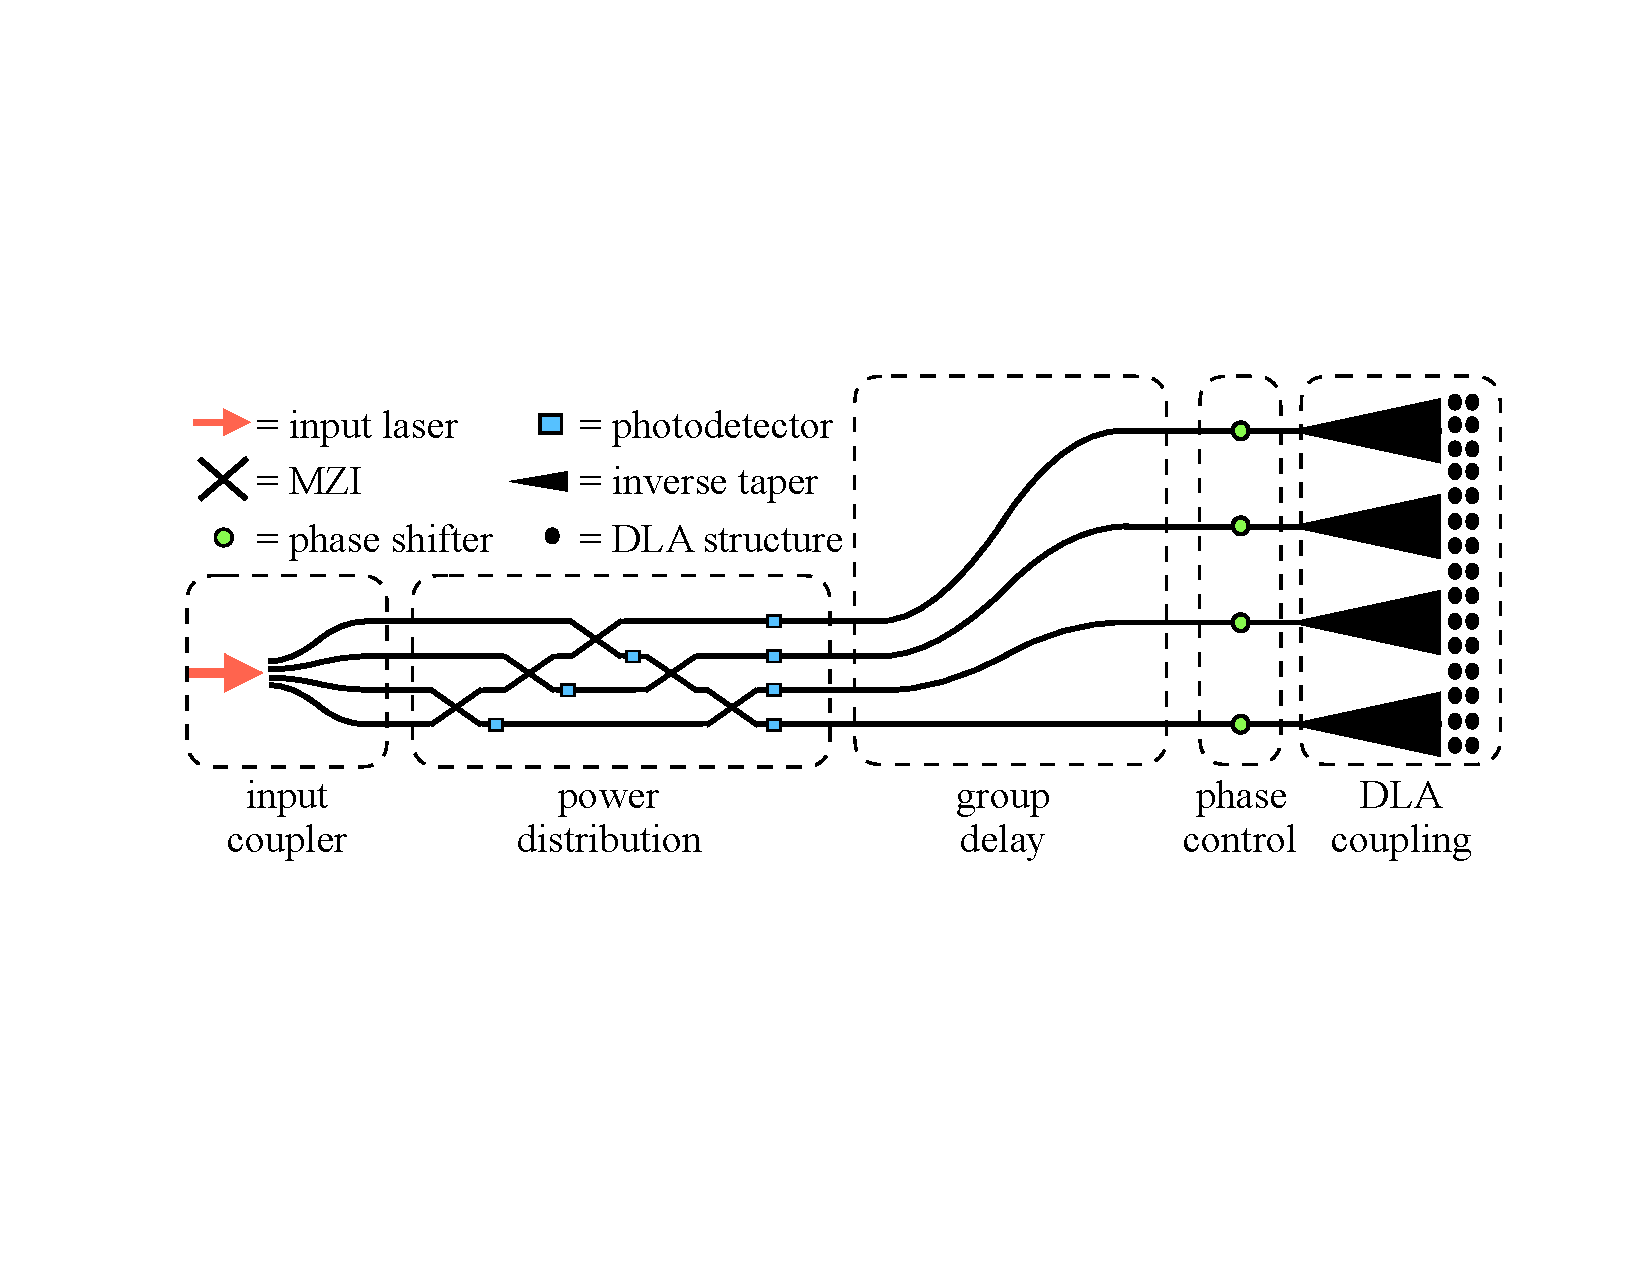
\includegraphics[width=1\columnwidth]{setup}
\caption{\label{fig:setup} Schematic of the proposed DLA laser delivery control system.  Although a one-sided input laser is shown, the same system may be operated in dual-drive mode with lasers incident from both sides \cite{leedle_phase-dependent_2018}.  In the system shown, the electron beam is traveling from bottom to top through the DLA structure gap on the right.  For a longer accelerator structure, more ports may be added to this configuration or it may be copied and reproduced along the vertical direction with each stage powered by its own phase-locked laser input source.}
\end{figure}

A schematic of our system is shown in Fig. \ref{fig:setup}.  The input coupling, power distribution, group delay (pulse-front tilt), phase control, and DLA coupling stages are performed separately.  Here we will give a brief overview of each stage before introducing the power distribution and phase control protocols in the next Sections.

\subsection{input coupling}
As mentioned, here we assume a `one-to-many' input coupling setup wherein a single laser beam is coupled directly into several dielectric waveguides.  However, our setup may also be applied to single-input coupling schemes, such as that explored in Ref. \cite{hughes_-chip_2017}.  One may to couple directly to several waveguides by focusing the laser beam directly onto several closely stacked end couplers (shown).  Alternatively, one could arrange an array of grating couplers on the surface of the chip, each with a corresponding waveguide output, and illuminate with an appropriately shaped laser beam.

\subsection{power distribution}
In this stage, we implement a partial MZI mesh for correcting the power distribution after the input coupling stage.  Each MZI, as represented by the waveguide crossings in Fig. \ref{fig:setup}, performs a unitary $2\times2$ operation on its inputs, which is tunable by two integrated optical phase shifters.  \cite{reck_experimental_1994,clements_optimal_2016,shen_deep_2017}.  After each MZI we include integrated photodetectors to measure the power coming out of each section.  This measurement is used as a signal for optimization in our power control procedure.  A similar setup was used for the mode sorter demonstration of Ref. \cite{annoni_unscrambling_2017}.

\subsection{group delay}
The purpose of this stage is to manipulate the laser pulse in each waveguide so that it arrives at the accelerator gap the same time as a moving electron beam. To do this, we introduce lithographically-defined bends in the waveguides to provide a group delay that is matched to the electron velocity, producing of the integrated optics analogue of a pulse-front tilt.  The mathematical details of the bend design are described in Ref. \cite{hughes_-chip_2017}.

\subsection{phase control}
This stage prepares the incoming laser pulse to ensure that it is in the proper phase for acceleration of the electron beam.  In Section \ref{sec:phase}, we show how one may do adaptive phase control using a downstream beam diagnostics setup involving successively measuring and adjusting each phase shifter in a systematic fashion.  While the phase shifters may be designed to maximize energy gain, they may also be designed to incorporate other metrics, such as beam focusing or total beam transmission, as long as these quantities may be measured downstream and these measurements used as a signal to optimize with.

\subsection{DLA coupling}
The final stage involves coupling the waveguide mode into the acceleration channel.  Ideally, an inverse taper or similar structure may be placed at the end of each waveguide to spread the mode area to match the geometry of the electron beam.  Then, an arbitrary accelerator structure may be placed adjacent to the end of the waveguides.  Alternatively, the accelerator structures and tapers may be part of the same system and may be designed following ideas from proposed buried grating structures \cite{chang_silicon_2014}, or using inverse design techniques, such as what was shown Ref. \cite{hughes_method_2017} for free-space coupling.

\begin{comment}
Fig. \ref{fig:setup}
\begin{figure*}
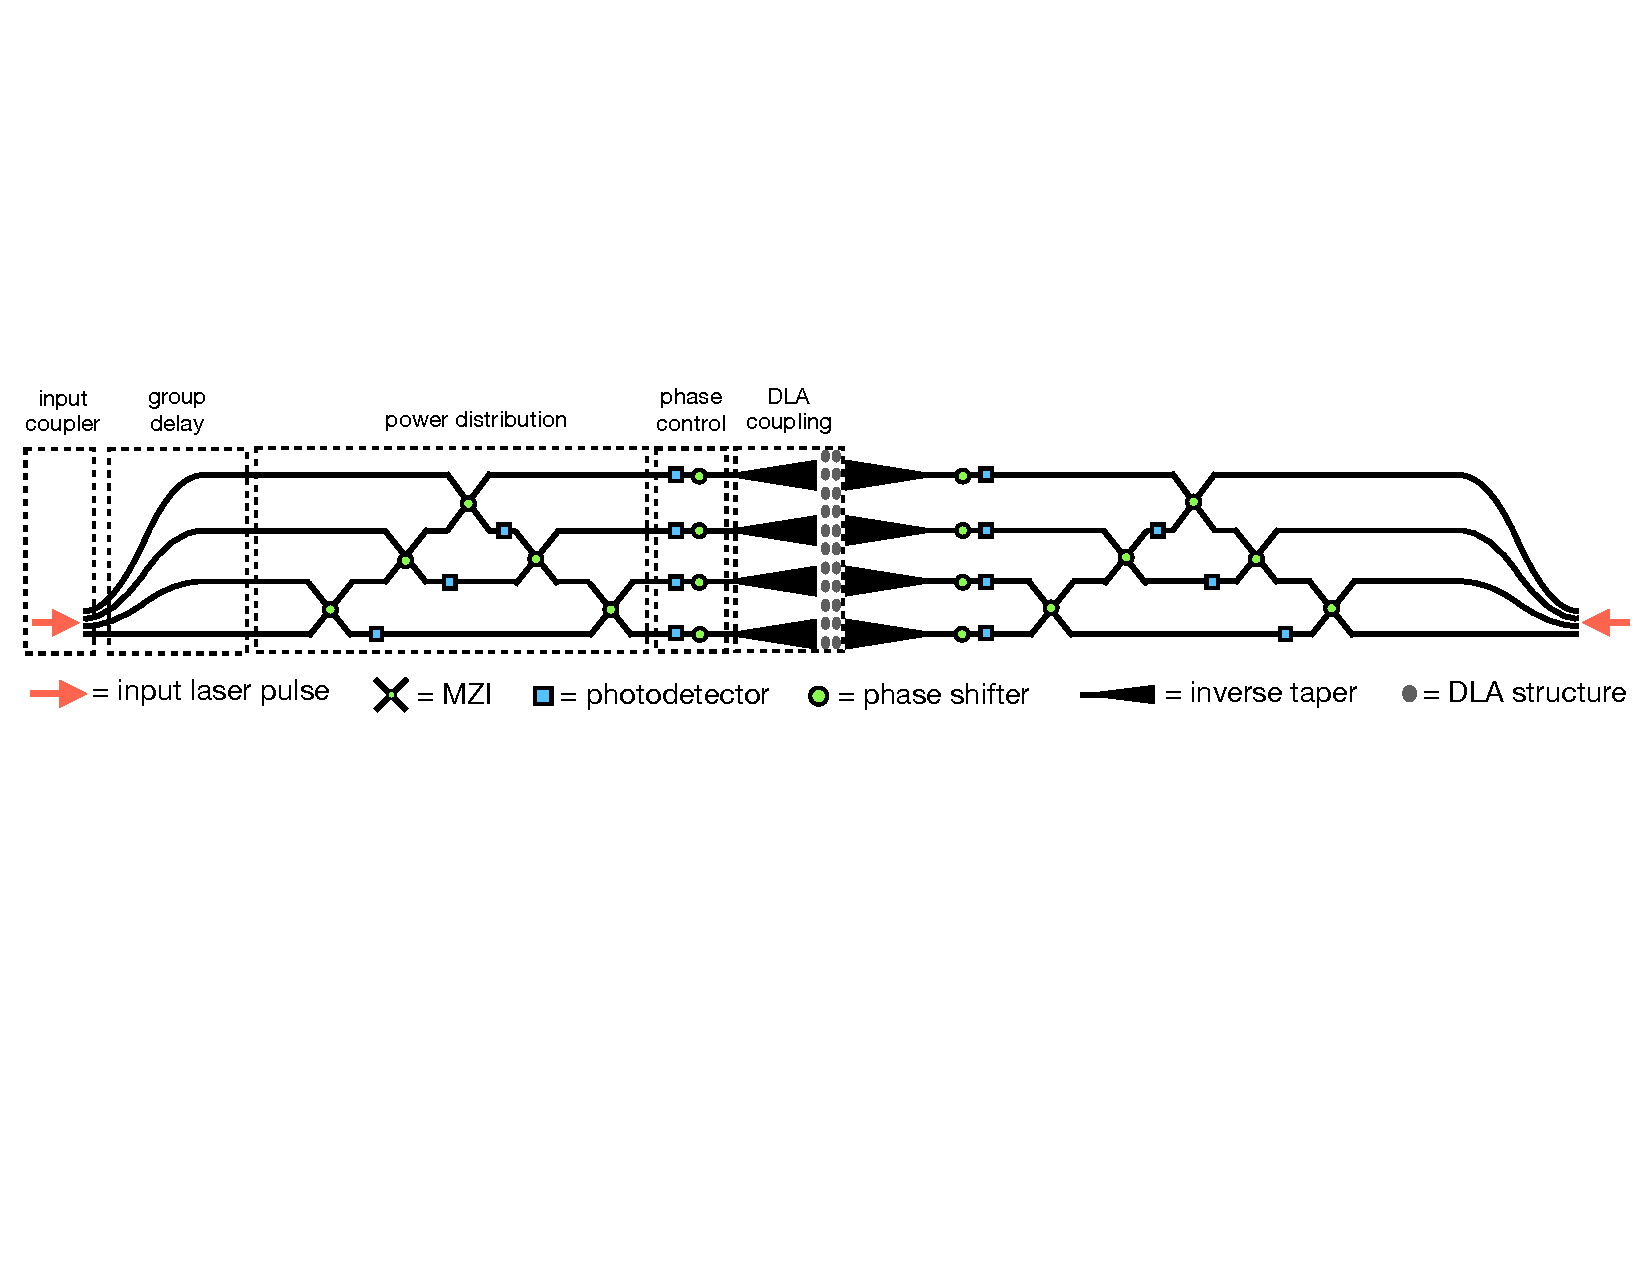
\includegraphics[width=1\textwidth]{setup_full}
\caption{\label{fig:setup} Setup}
\end{figure*}
\end{comment}

\section{\label{sec:power}Power distribution protocol}

%Fig. \ref{fig:norm}
%
%\begin{figure}
%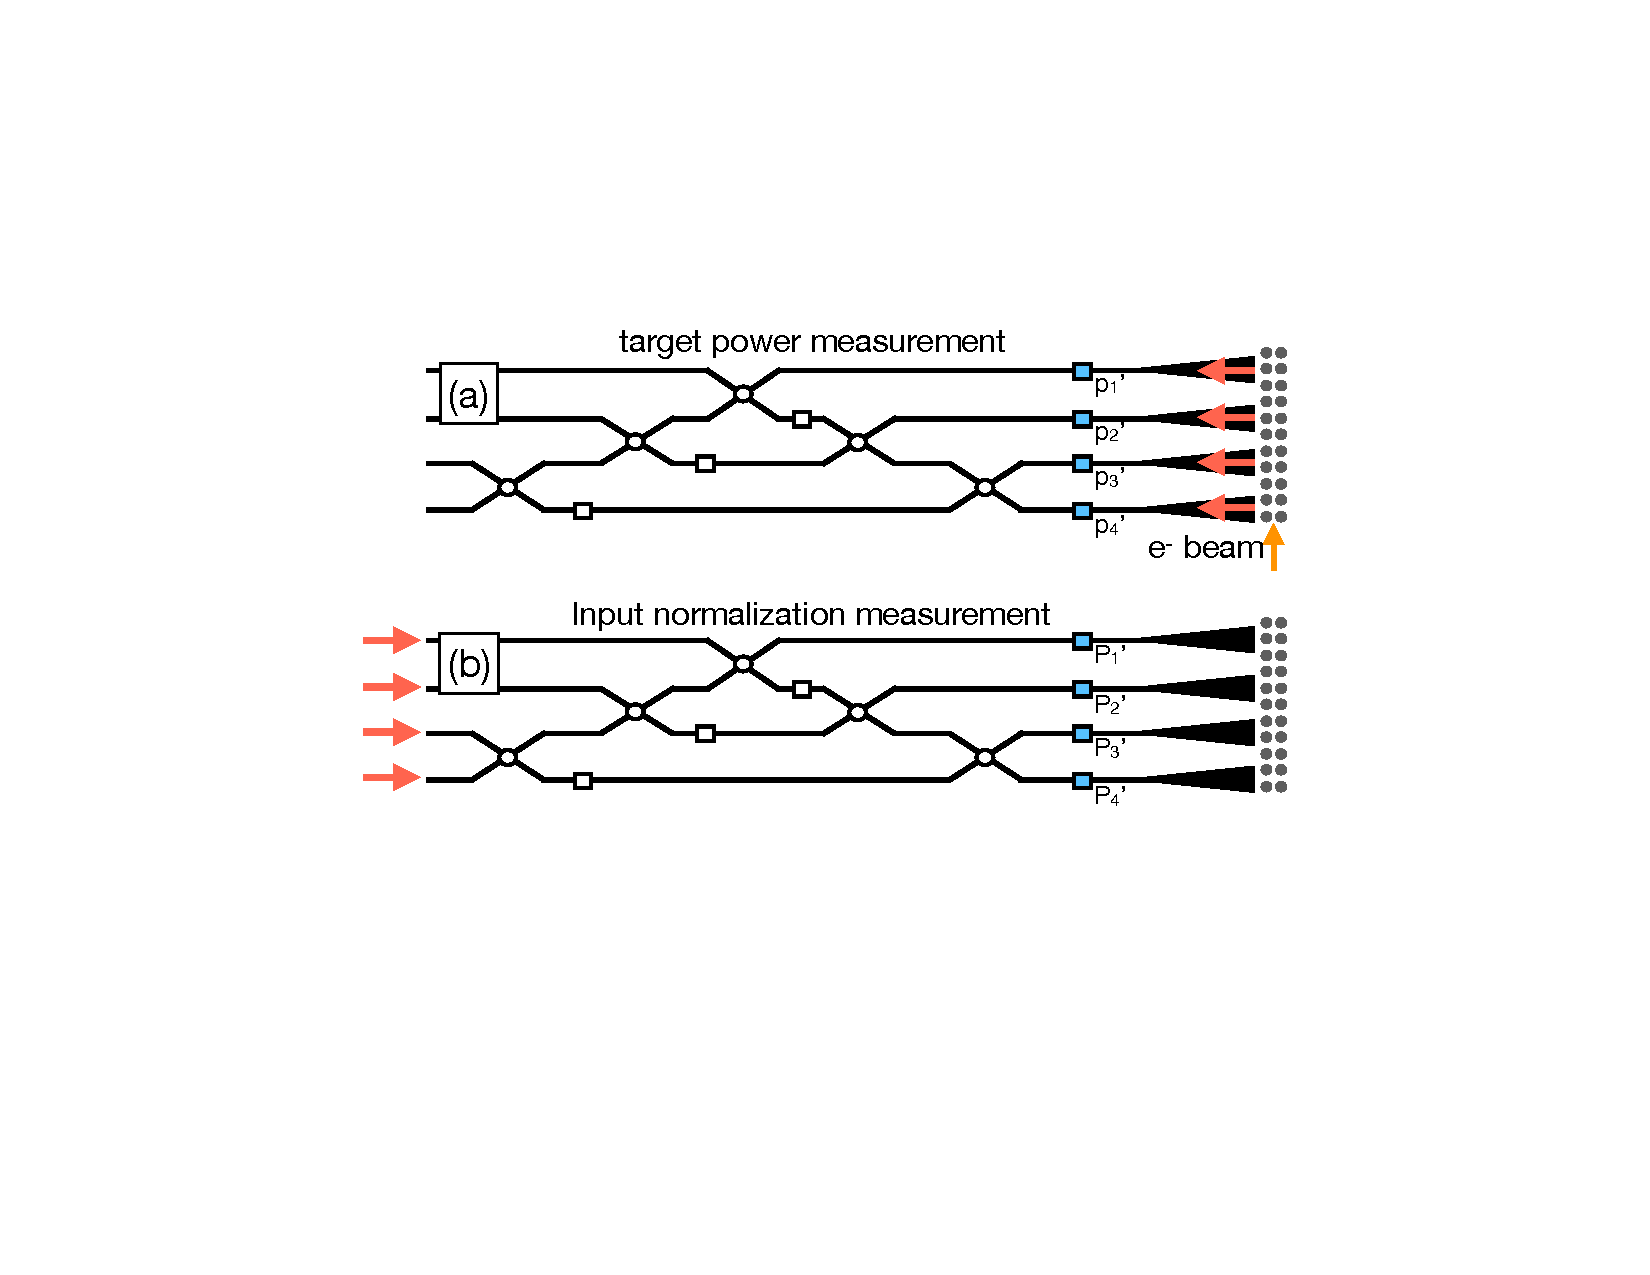
\includegraphics[width=0.78\columnwidth]{normalization}
%\caption{\label{fig:norm} Normalization}
%\end{figure}

Fig. \ref{fig:power}

\begin{figure}
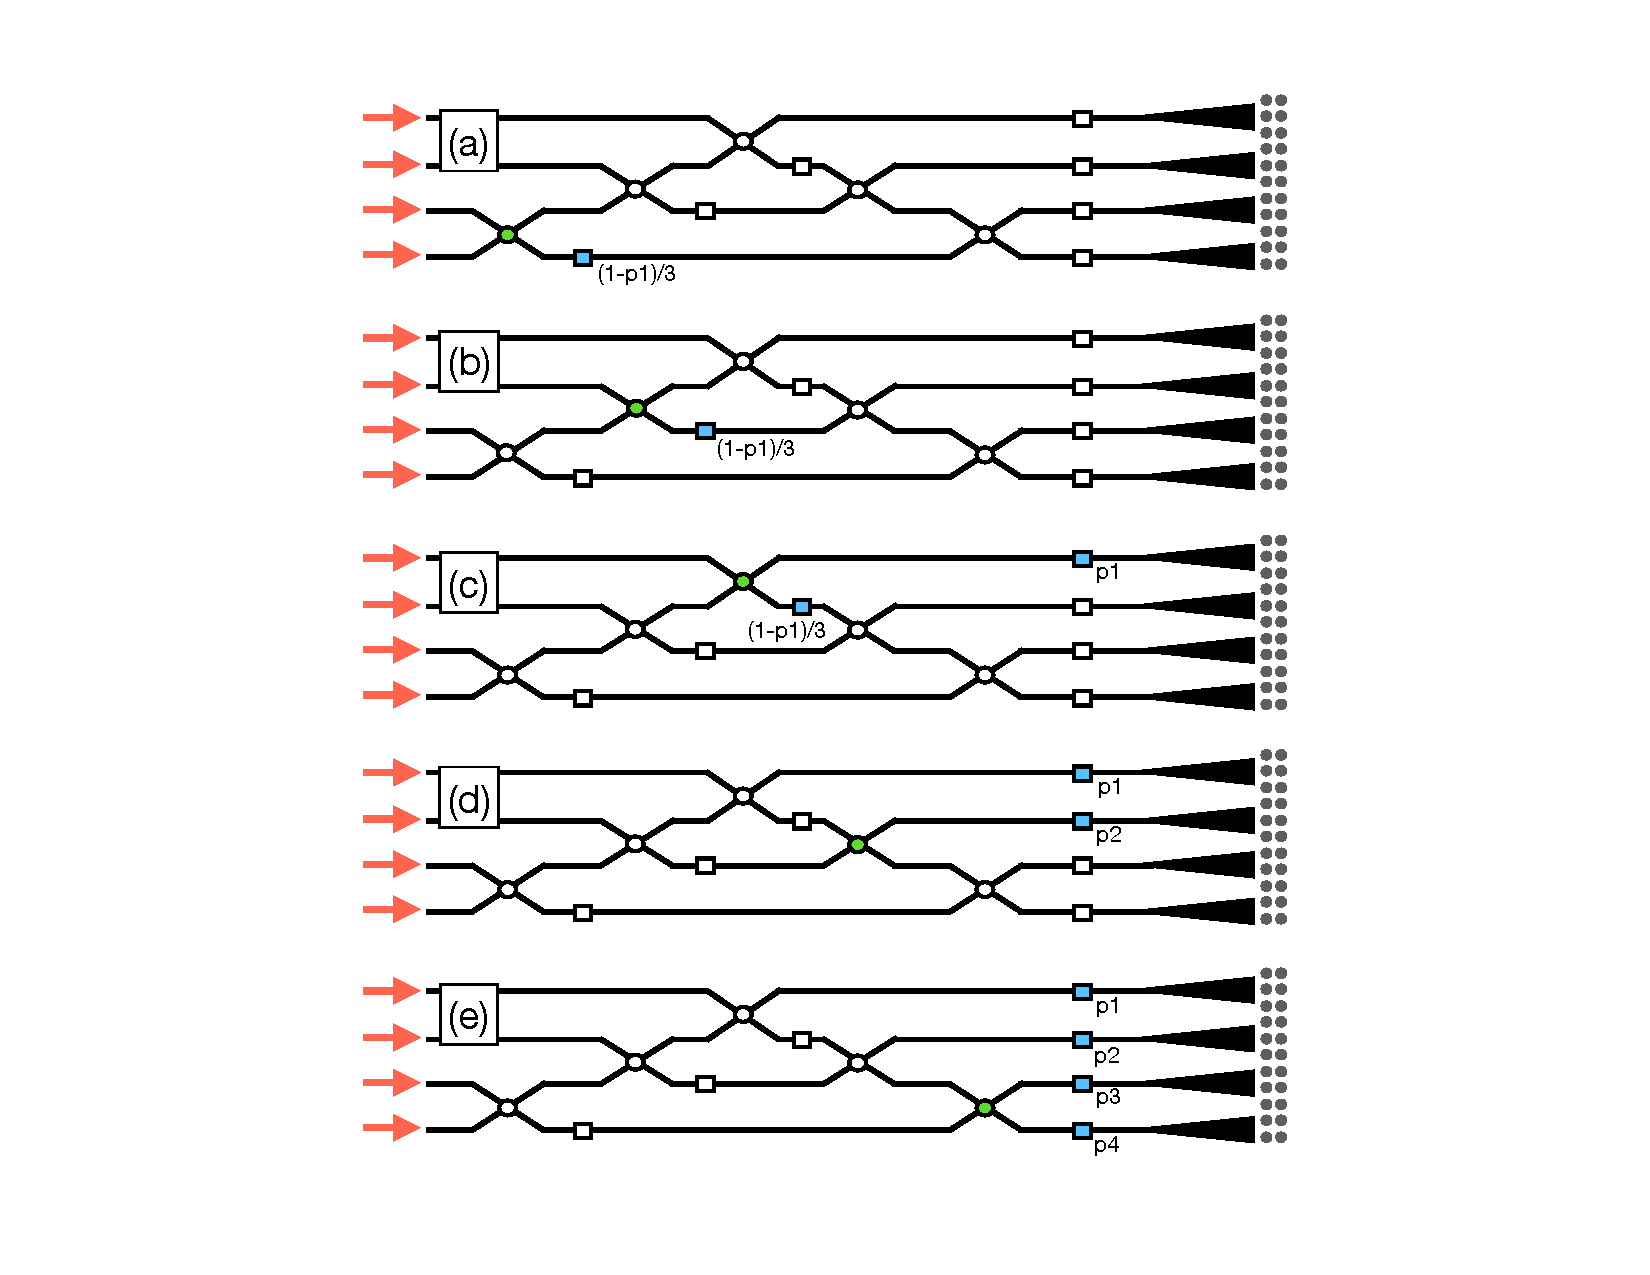
\includegraphics[width=0.8\columnwidth]{amplitude_tuning}
\caption{\label{fig:power} Power distribution}
\end{figure}

\section{\label{sec:phase}Phase control}

Now that power is distributed, can do phase control.

System in Fig. \ref{fig:phase}.

Need spectrometer upstream to optimize the final phase shifters with respect to electron energy gain.

Could be interested in other quantities, such as total electron transmission.

Beam diagnostic can be accomplished with on-chip components [cite ken soong's beam position monitor]

May implement switches to dump the port to grating couplers, see Fig. \ref{fig:phase}.
\begin{figure}
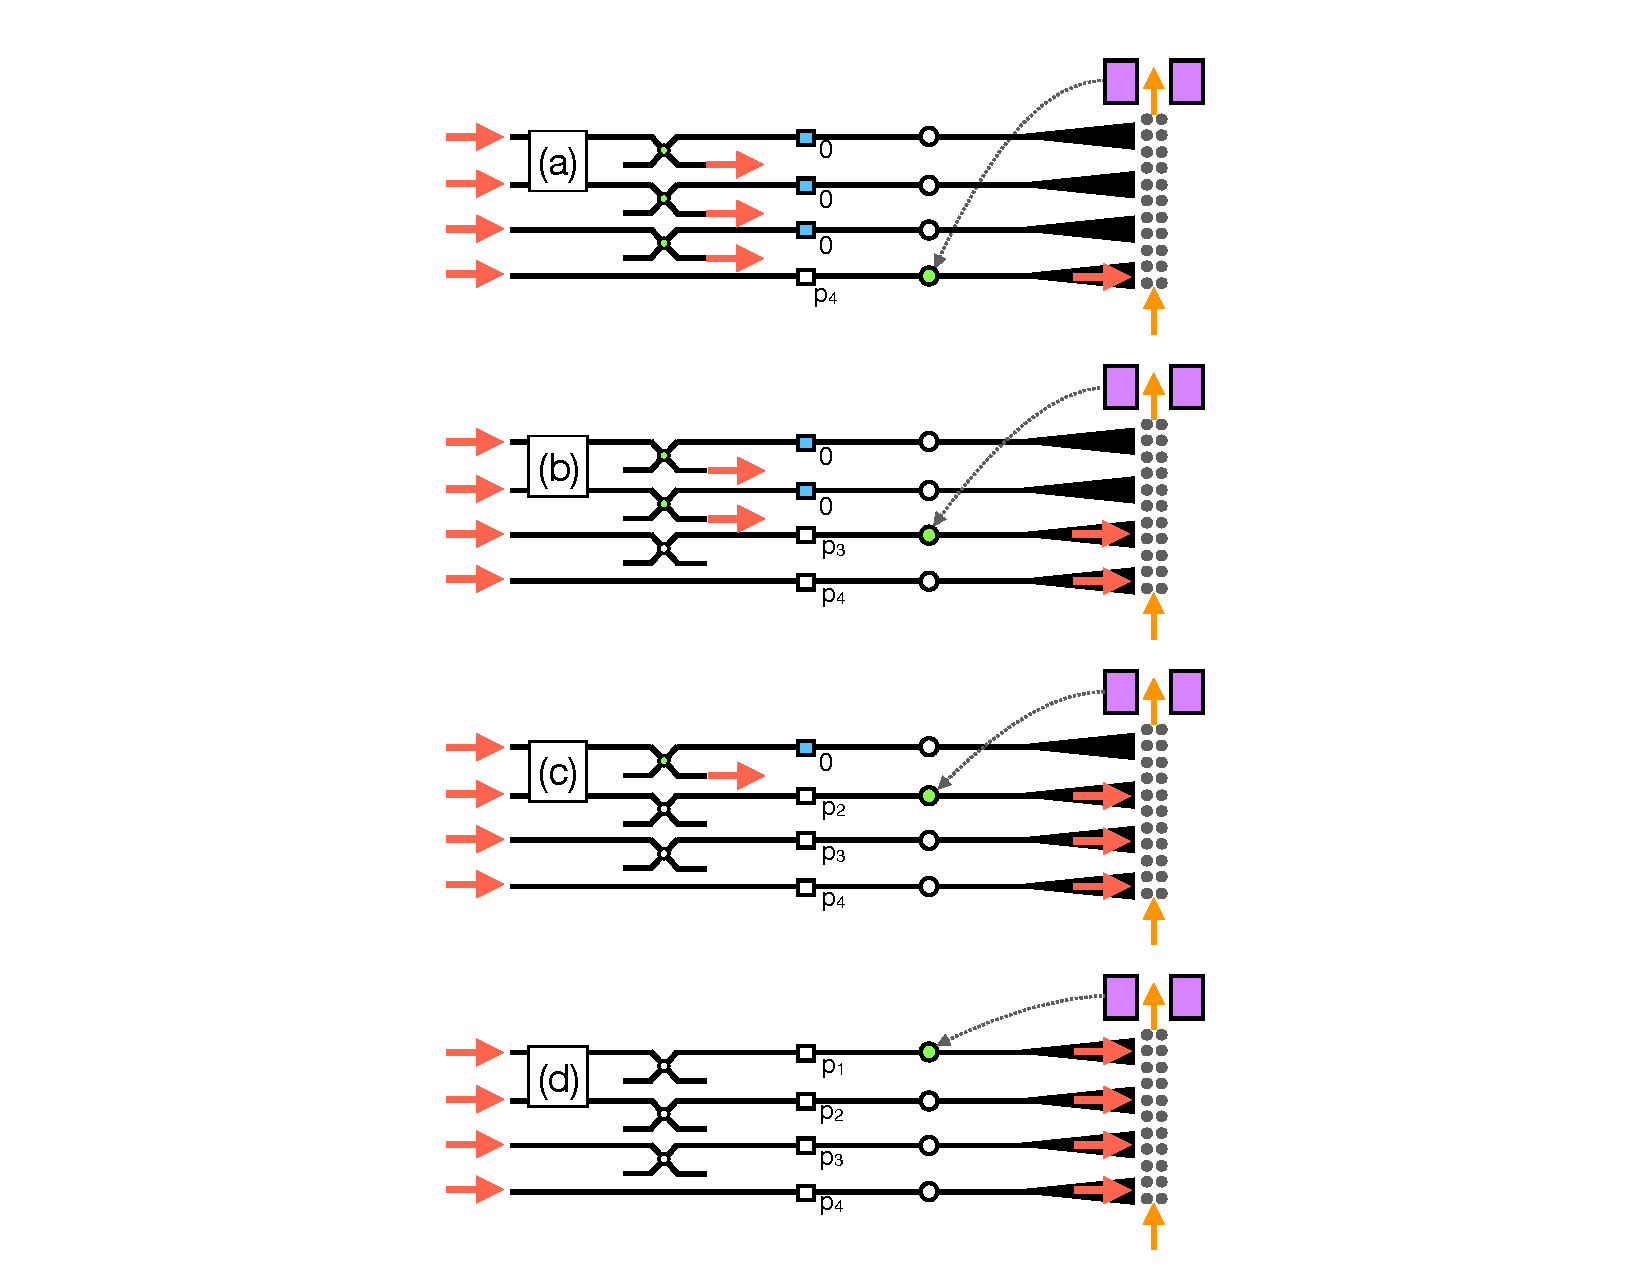
\includegraphics[width=0.75\columnwidth]{phase_tuning}
\caption{\label{fig:phase} Phase tuning}
\end{figure}

\section{\label{sec:demo}Demonstration}

cite [reck, clemson] for how device is parameterized.

Use gradient descent with numerical gradient with respect to phase shifters in MZI.

Approximately linear scaling with number of layers.

(Code available at link)

Fig. \ref{fig:demo}

\begin{figure}
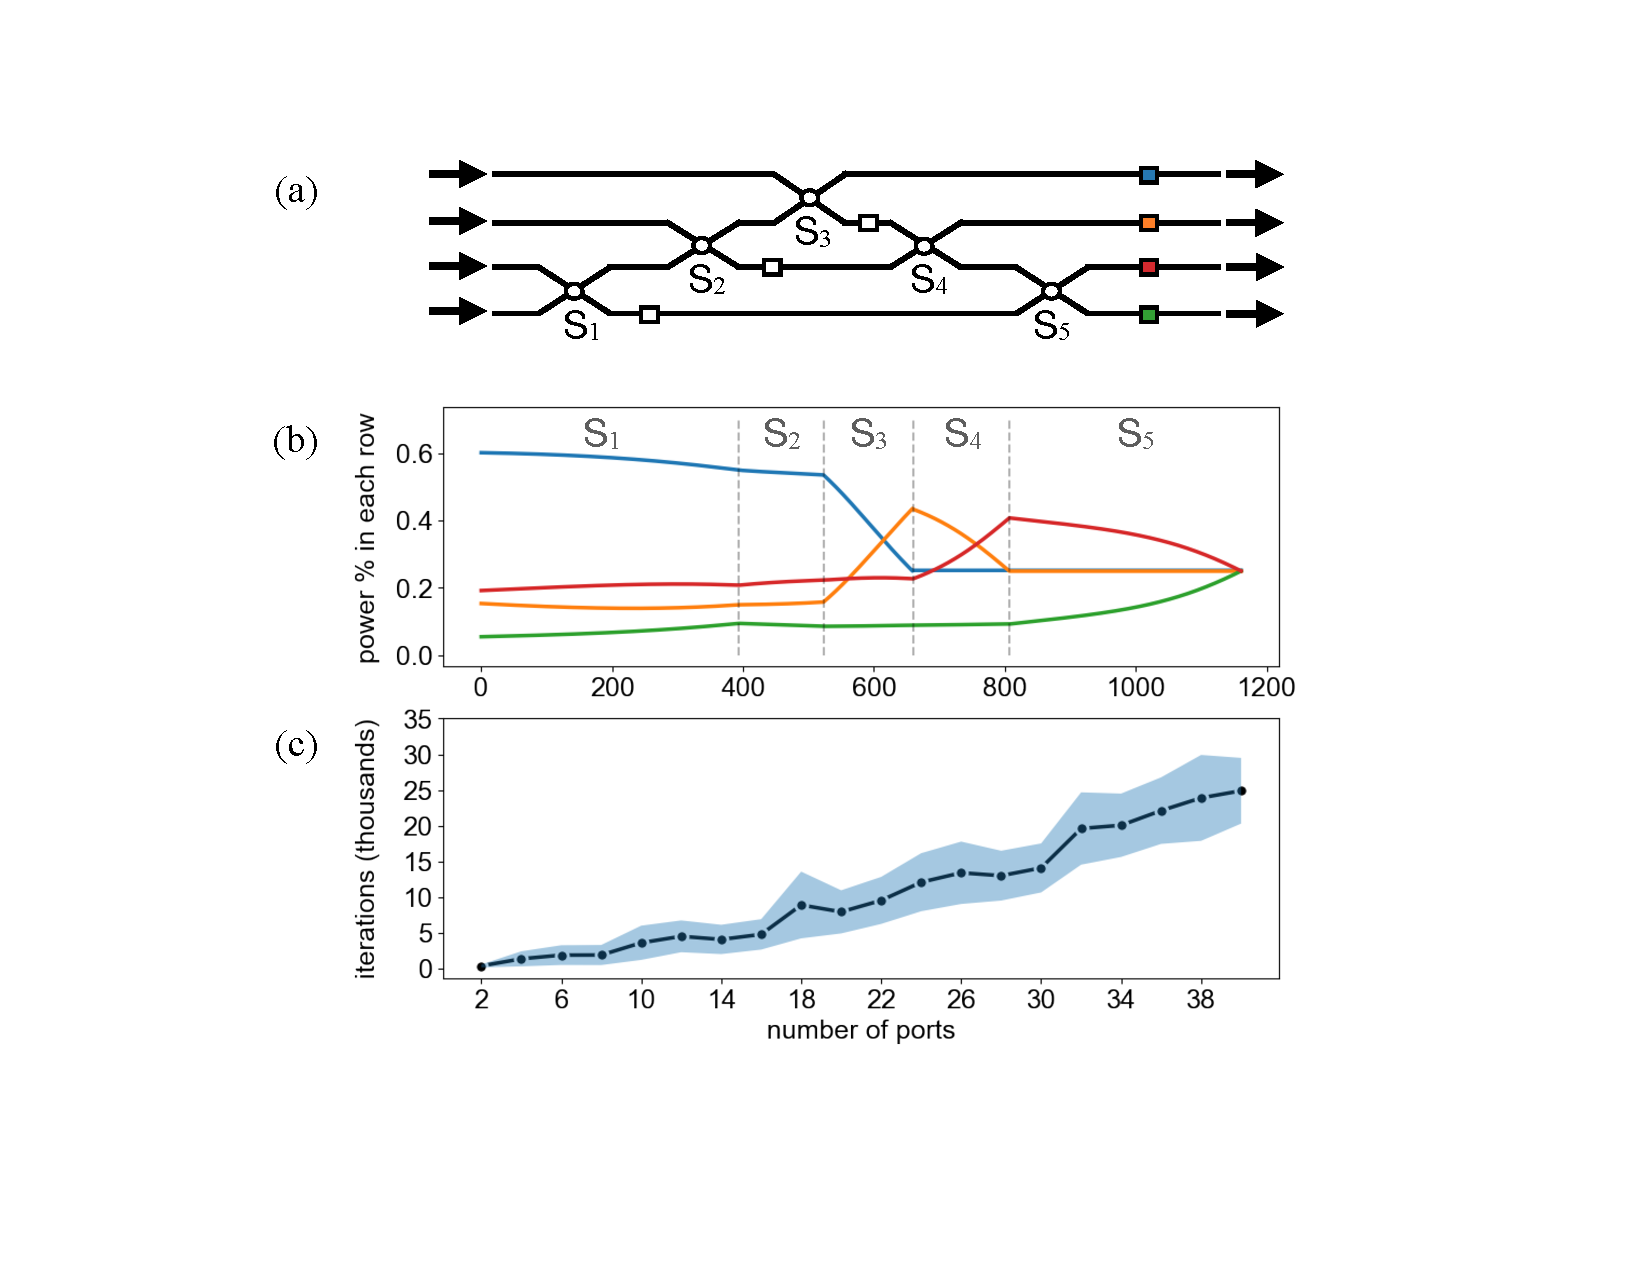
\includegraphics[width=1\columnwidth]{demo}
\caption{\label{fig:demo} Demonstration}
\end{figure}

\section{\label{sec:discussion}Discussion}
1. \textbf{Major findings}

- MZI meshes are promising candidates for DLA power delivery and control.  No new components necessary, scaling demonstrated to be highly favorable for large systems.

- Through AVM, we see that electron beam may be used as a diagnostic tool for both efficient coupling and phase tuning.

2. \textbf{What is new and novel}

- While components are not new, the procedure is novel and tailored to the unique requirements of DLA (high power, short pulses, amplitude and phase control, group velocity delay).

3. \textbf{How does it compare with literature?}

- Compared to mode sorters, expect similar performance.  

- With other things, such as ANNs and QIP setups, have very different requirements and constraints.  (talk about ANN training?)

4. \textbf{What are the limitations?}

- Bandwidth of MZIs vs. bandwidth of pulse.
 
- Maintaining group velocity delay in structure, (need to add additional `dummy' MZIs?)

- Technical implementation, need for several phase shifters, photodetectors, and associated electronics in vacuum with DLA.

5. \textbf{Implications/future work}

- Integrated optical power delivery systems are worth continuing to pursue for DLA.

- Path forward involves experimentally demonstrating 1 (phase only), 2 (phase + amplitude), and more stages of waveguide powered DLA with this mechanism for control.

- Optical control of phase shifters and power measurements through optical scattering may be considered as a simplification strategy.

- New waveguide-based beam diagnostic elements beam position monitors and electron spectrometers should be considered.

- de-focusing may be corrected by using this setup to implement alternative focusing schemes, which require control over the input phase and amplitude along device. ponderomotive focusing [naranjo] or alternating phase focusing [swenson, cohen]

\section{\label{sec:conclusion}Conclusion}
1. \textbf{What you did/introduced}

- Introduce MZI mesh as a tool for DLA power delivery and control system.

- Give systematic procedure for doing both power distribution and phase control using only power measurements in the device and use of integrated optical phase shifters.

- Show that this may effectively tune DLA structures with a reasonable time scaling.

2. \textbf{The result (numbers)}

- Estimate that for an assumed $L mm$ long structure with $N$ stages, we can tune in $s$ seconds using $p$-class of phase shifters.

3. \textbf{The outcome/take-home message}

- Integrated optics, and reconfigurable optics in general, allows unique opportunities for DLA to take advantage of high precision control and adaptability.

- This is a very promising avenues for accomplishing extended acceleration lengths and eventually targeting applications with DLA technology.

\begin{comment}
\appendix

\section{\label{appx} Numerical Simulation Model}

Here we give details on the mathematics of the simulation from Section \ref{sec:demo}.  We show how the power distribution stage is performed on a system with $N$ total input and output ports.  It follows that, without loss or backscattering, the system may be described by a $N \times N$, unitary matrix, `$M$', where $M_{i,j}$ relates the modal amplitude at input port $j$ to the modal amplitude at output port $i$.  

As there are $2N-3$ MZIs in the system, the matrix $M$ is constructed by successively multiplying $2N-3$ corresponding $N \times N$ matrices correpsonding to each MZI.  With these MZI matrices labelled $M_i$ for $i = 1...2N-3$ from left to right, 
\begin{equation}
M = \prod_{i=2N-3}^1 M_i.
\end{equation}

Here $M_i$ is matrix with ones along its diagonal and a $2 \times 2$ matrix, $B$, corresponding to the MZI, embedded at an index that corresponds to the $i$-th MZI's position in the network.  For an example, 

\begin{equation}
M_1 = 
\begin{bmatrix}
	1 & 0      & 0 &        &  0       & 0       \\
	0 & 1      & 0 & \cdots &  0       & 0       \\
	0 & 0      & 1 &        &  0       & 0       \\
	  & \vdots &   &        &  0       & 0       \\
	0 & 0      & 0 &    0   &  B_{1,1} & B_{1,2} \\
	0 & 0      & 0 &    0   &  B_{2,1} & B_{2,2}
\end{bmatrix}
\end{equation}

Where, $B$ is parameterized by the phase of each of the integrated phase shifters in the MZI, $\phi_1$ and $\phi_2$ as
\begin{equation}
B(\phi_1,\phi_2) = -ie^{i\phi_2/2}
\begin{bmatrix}
  -\sin(\phi_2/2) & \cos(\phi_2/2)e^{i\phi_1} \\
  \cos(\phi_2/2) & \sin(\phi_2/2)e^{i\phi_1}
\end{bmatrix}.
\end{equation}
\end{comment}
\bibliography{DLA_Phase_Control}
\end{document}